% =============================================================================
% BioBoard EEG System — Architecture Documentation
% =============================================================================
\documentclass[11pt,a4paper]{article}

% --- Packages ---
\usepackage[utf8]{inputenc}
\usepackage[T1]{fontenc}
\usepackage{lmodern}
\usepackage[margin=2.0cm]{geometry}
\usepackage{graphicx}
\usepackage{xcolor}
\usepackage{booktabs}
\usepackage{tabularx}
\usepackage{array}
\usepackage{multirow}
\usepackage{makecell}
\usepackage{amsmath}
\usepackage{amssymb}
\usepackage{enumitem}
\usepackage{listings}
\usepackage{float}
\usepackage{caption}
\usepackage{textcomp}
\usepackage{hyperref}
\usepackage{cleveref}
\usepackage{tikz}
\usepackage{fancyhdr}
\usepackage{titlesec}
\usepackage{longtable}

% --- TikZ libraries ---
\usetikzlibrary{arrows.meta, positioning, shapes.geometric, shapes.multipart,
                 fit, calc, backgrounds, decorations.pathmorphing}

% --- Colours ---
\definecolor{hwcolor}{HTML}{1565C0}     % hardware blue
\definecolor{fwcolor}{HTML}{2E7D32}     % firmware green
\definecolor{conncolor}{HTML}{E65100}   % connector orange
\definecolor{plugincolor}{HTML}{6A1B9A} % plugin purple
\definecolor{oecolor}{HTML}{C62828}     % Open Ephys red
\definecolor{extcolor}{HTML}{37474F}    % external grey
\definecolor{infracolor}{HTML}{546E7A}  % infrastructure / transport
\definecolor{codebg}{HTML}{F5F5F5}
\definecolor{codeframe}{HTML}{BDBDBD}

% --- Listings ---
\lstset{
    basicstyle=\ttfamily\small,
    backgroundcolor=\color{codebg},
    frame=single,
    rulecolor=\color{codeframe},
    breaklines=true,
    tabsize=4,
    showstringspaces=false,
    captionpos=b
}

% --- Header / footer ---
\pagestyle{fancy}
\fancyhf{}
\fancyhead[L]{\small BioBoard EEG System Architecture DRAFT}
\fancyhead[R]{\small v0.1 — \today}
\fancyfoot[L]{\small Document ID: Pending}
\fancyfoot[C]{\thepage}

% --- Section formatting ---
\titleformat{\section}{\large\bfseries\color{hwcolor}}{\thesection}{1em}{}
\titleformat{\subsection}{\normalsize\bfseries\color{hwcolor!80!black}}{\thesubsection}{1em}{}
\titleformat{\subsubsection}{\normalsize\bfseries\color{hwcolor!60!black}}{\thesubsubsection}{1em}{}

% --- Custom commands ---
\newcommand{\component}[1]{\texttt{\textbf{#1}}}
\newcommand{\proto}[1]{\textsc{#1}}
\newcommand{\reg}[1]{\texttt{#1}}
\newcommand{\hex}[1]{\texttt{0x#1}}

% =============================================================================
\begin{document}

\begin{center}
    {\LARGE\bfseries In-Ear System Architecture Documentation --- DRAFT} \\[0.5em]
    {\small Version 0.1 \quad---\quad \today}
\end{center}

\vspace{1em}
\begin{table}[H]
\centering
\caption*{\large\bfseries\color{hwcolor}Document Control}
\begin{tabularx}{0.9\textwidth}{|>{\bfseries}l|X|}
\hline
Document ID & Pending \\
 \hline
Version & 0.1 \\
 \hline
Status & Draft \\
 \hline
Prepared by & Polymer Bionics Limited \\
 \hline
Approved by & \\
 \hline
Approval Date & \\
 \hline
Review Date & \\
\hline
\end{tabularx}
\end{table}

\vspace{0.8em}
\begin{table}[H]
\centering
\caption*{\large\bfseries\color{hwcolor}Revision History}
\begin{tabularx}{0.9\textwidth}{|l|l|l|X|}
\hline
\textbf{Version} & \textbf{Date} & \textbf{Author} & \textbf{Summary} \\
\hline
0.1 & \today & Polymer Bionics Limited & Initial draft issued for internal review and QMS approval. \\
\hline
\end{tabularx}
\end{table}

\newpage
\tableofcontents
\vspace{1.5em}
\newpage

% =============================================================================
\section{System Overview}
% =============================================================================

The BioBoard is a modular, \textbf{platform-agnostic} biosignal acquisition
platform built around the \textbf{Teensy~4.1} and \textbf{TI ADS1299}
24-bit EEG front-end.  A \textbf{standalone Qt Connector App} bridges
hardware to \textbf{Lab Streaming Layer (LSL)}, enabling any LSL-compatible
software (OpenBCI GUI, MATLAB, LabRecorder, etc.)
to consume the data.

Four architectural layers:

\begin{enumerate}[leftmargin=2cm]
    \item[\textcolor{hwcolor}{\textbf{L1}}] \textbf{Hardware} — Teensy~4.1 + ADS1299 + sensors
    \item[\textcolor{fwcolor}{\textbf{L2}}] \textbf{Firmware} — Compact Protocol v1.0 over USB serial
    \item[\textcolor{conncolor}{\textbf{L3}}] \textbf{Connector} — Qt Connector App (USB $\to$ LSL)
    \item[\textcolor{plugincolor}{\textbf{L4}}] \textbf{Consumers} — Open Ephys and any other LSL-compatible software
\end{enumerate}

\subsection{End-to-End Data Flow}

Primary production path (recommended):

\begin{itemize}
    \item \textbf{Connector-first path:} Qt Connector App reads serial data and
          publishes LSL streams directly. Open Ephys can then subscribe as an
          LSL consumer (same as MATLAB, Python, LabRecorder, etc.).
    \item \textbf{Single-parser architecture:} No direct firmware $\rightarrow$ Open Ephys
          serial path in the primary design. This avoids maintaining two separate
          protocol parsers (Connector + Open Ephys).
    \item \textbf{Event round-trip (optional):} Open Ephys can publish markers/events
          back into LSL (e.g., Paradigm Bridge), while external tools such as
          PsychoPy can also publish behavioral/event streams to LSL.
\end{itemize}

\begin{figure}[H]
\centering
\resizebox{\linewidth}{!}{%
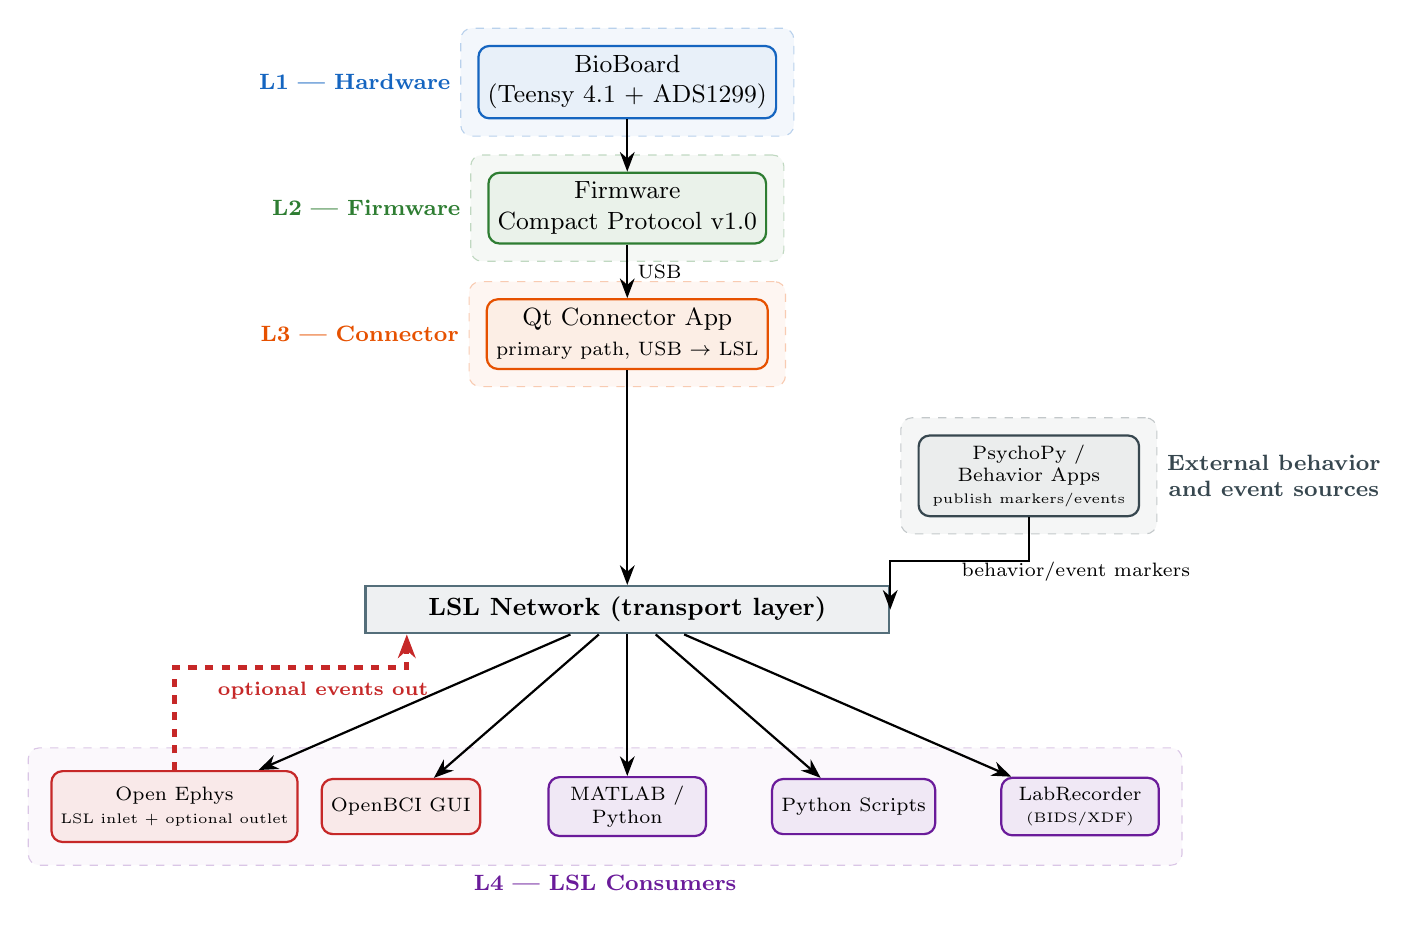
\begin{tikzpicture}[
    every node/.style={font=\small, align=center},
    hw/.style={draw=hwcolor, fill=hwcolor!10, rounded corners, thick,
               minimum width=3.2cm, minimum height=0.8cm},
    fw/.style={draw=fwcolor, fill=fwcolor!10, rounded corners, thick,
               minimum width=3.2cm, minimum height=0.8cm},
    conn/.style={draw=conncolor, fill=conncolor!10, rounded corners, thick,
                 minimum width=3.2cm, minimum height=0.8cm},
    lslbus/.style={draw=infracolor, fill=infracolor!10, thick,
                   minimum width=6.65cm, minimum height=0.6cm,
                   font=\small\bfseries},
    consumer/.style={draw=plugincolor, fill=plugincolor!10, rounded corners, thick,
                     minimum width=2cm, minimum height=0.7cm,
                     font=\scriptsize},
    oeconsumer/.style={draw=oecolor, fill=oecolor!10, rounded corners, thick,
               minimum width=2.6cm, minimum height=0.9cm,
               font=\scriptsize},
    extsrc/.style={draw=extcolor, fill=extcolor!10, rounded corners, thick,
                   minimum width=2.8cm, minimum height=0.75cm,
                   font=\scriptsize},
    arr/.style={-{Stealth[length=2.5mm]}, thick}
]
    % Row 0: Hardware
    \node[hw] (bio) at (0, 0) {BioBoard\\(Teensy~4.1 + ADS1299)};

    % Row 1: Firmware
    \node[fw] (fw) at (0, -1.6) {Firmware\\Compact Protocol v1.0};

    % Connector (primary path)
    \node[conn] (qt) at (0, -3.2) {Qt Connector App\\{\scriptsize primary path, USB $\to$ LSL}};

    % LSL bus (transport/infrastructure, not an L4 consumer)
    \node[lslbus] (lsl) at (0, -6.7) {LSL Network (transport layer)};

    % External behavior/event source
    \node[extsrc] (psy) at (5.1, -5.0) {PsychoPy /\\Behavior Apps\\{\tiny publish markers/events}};

    % Consumers
    \node[oeconsumer] at (-5.75, -9.2) (oein) {Open Ephys\\{\tiny LSL inlet + optional outlet}};
    \node[consumer, draw=oecolor, fill=oecolor!10] at (-2.875, -9.2) (obci)   {OpenBCI GUI};
    \node[consumer] at (0, -9.2)    (matlab) {MATLAB /\\Python};
    \node[consumer] at (2.875, -9.2)  (mne)    {Python Scripts};
    \node[consumer] at (5.75, -9.2)  (labrec) {LabRecorder\\{\tiny (BIDS/XDF)}};

    % Arrows — top
    \draw[arr] (bio) -- (fw);

    % Arrows — primary path
    \draw[arr] (fw) -- node[right, font=\scriptsize] {USB} (qt);
    \draw[arr] (qt) -- (lsl);

    % Arrows — external behavior/event source to LSL
    \draw[arr] (psy.south) -- ++(0,-0.55) -| (lsl.east)
          node[pos=0.28, right, yshift=-4pt, font=\scriptsize] {behavior/event markers};

    % Arrows — consumers
    \draw[arr] (lsl) -- (oein);
    \draw[arr] (lsl) -- (obci);
    \draw[arr] (lsl) -- (matlab);
    \draw[arr] (lsl) -- (mne);
    \draw[arr] (lsl) -- (labrec);
    \draw[-{Stealth[length=3mm]}, line width=1.8pt, draw=oecolor, dashed]
          (oein.north) -- ++(0,1.3) -| ([xshift=-2.8cm]lsl.south)
          node[pos=0.32, below=1pt, font=\scriptsize\bfseries, text=oecolor]
          {optional events out};

    % Background labels
    \begin{scope}[on background layer]
        \node[fit=(bio), inner sep=6pt, fill=hwcolor!5, draw=hwcolor!30,
              dashed, rounded corners,
              label={[hwcolor, font=\footnotesize\bfseries]left:L1 — Hardware}] {};
        \node[fit=(fw), inner sep=6pt, fill=fwcolor!5, draw=fwcolor!30,
              dashed, rounded corners,
              label={[fwcolor, font=\footnotesize\bfseries]left:L2 — Firmware}] {};
        \node[fit=(qt), inner sep=6pt, fill=conncolor!5, draw=conncolor!30,
              dashed, rounded corners,
              label={[conncolor, font=\footnotesize\bfseries]left:L3 — Connector}] {};
        \node[fit=(psy), inner sep=6pt, fill=extcolor!5,
              draw=extcolor!30, dashed, rounded corners,
              label={[extcolor, font=\footnotesize\bfseries]right=4pt:External behavior\\and event sources}] {};
        \node[fit=(oein)(obci)(matlab)(mne)(labrec), inner sep=8pt,
              fill=plugincolor!3, draw=plugincolor!25, dashed, rounded corners,
              label={[plugincolor, font=\footnotesize\bfseries]below:L4 — LSL Consumers}] {};
    \end{scope}
\end{tikzpicture}}% end resizebox
\caption{Primary architecture: Qt Connector App is the single serial parser and
         publishes LSL streams consumed by Open Ephys and other tools. External
         behavior/event tools (e.g., PsychoPy) can publish markers to LSL, and
         Open Ephys can optionally publish events back to LSL (dashed). The LSL
         network is transport infrastructure, not an L4 consumer.}
\label{fig:system-overview}
\end{figure}


% =============================================================================
\section{Layer 1 — Hardware (BioBoard)}
\label{sec:hardware}
% =============================================================================

\subsection{Core Components}

\begin{table}[H]
\centering
\caption{BioBoard hardware components}
\label{tab:hw-components}
\begin{tabularx}{\textwidth}{l l X}
\toprule
\textbf{Component} & \textbf{Manufacturer / Part} & \textbf{Function} \\
\midrule
MCU          & Teensy~4.1 (ARM Cortex-M7, 600\,MHz)
             & Main controller; USB 2.0 Full Speed \\
EEG ADC      & \makecell[l]{Texas Instruments\\ADS1299\\\href{https://www.ti.com/lit/gpn/ads1299}{datasheet}}
             & Biosignal front-end; SPI interface; configurable gain 1$\times$--24$\times$ \\
Accelerometer & \makecell[l]{Analog Devices, Inc.\\ADXL367\\\href{https://www.analog.com/media/en/technical-documentation/data-sheets/adxl367.pdf}{datasheet}}
             & Motion/orientation; low-noise MEMS \\
PPG / SpO$_2$ & \makecell[l]{Analog Devices, Inc.\\MAXM86161\\\href{https://www.analog.com/media/en/technical-documentation/data-sheets/maxm86161.pdf}{datasheet}}
             & Integrated PPG + SpO$_2$; single optical module \\
Temperature  & \makecell[l]{Texas Instruments\\TMP117\\\href{https://www.ti.com/lit/gpn/tmp117}{datasheet}}
             & High-precision digital temperature sensor \\
Connection   & USB 2.0
             & Serial at 2\,Mbaud (2\,000\,000\,bps) \\
\bottomrule
\end{tabularx}
\end{table}


% =============================================================================
% FIRMWARE SECTION — commented out for now
% =============================================================================
\iffalse

\begin{table}[H]
\centering
\caption{Compact Protocol v1.0 parameters}
\label{tab:proto-params}
\begin{tabularx}{\textwidth}{l X}
\toprule
\textbf{Parameter} & \textbf{Value} \\
\midrule
EEG Sample Rate      & 1000\,Hz \\
EEG Channels         & 8 (24-bit signed, 24\,B total) \\
Baud Rate            & 2\,000\,000 (2\,Mbaud) \\
Byte Order           & Big-Endian (network order) \\
Packet Size          & 32--38\,B (variable, depends on auxiliary payload) \\
Best Case (EEG only) & 32\,B \\
Worst Case (EEG + Accel) & 38\,B \\
Fixed Overhead       & 8\,B (7\,B header + 1\,B checksum) \\
Error Detection      & XOR checksum (1\,B) \\
\bottomrule
\end{tabularx}
\end{table}

\subsection{Packet Structure}

\begin{lstlisting}
START(2B) | TIMESTAMP(4B) | TYPE+TTL(1B) | EEG(24B) | [AUX] | CHECKSUM(1B)
\end{lstlisting}

\subsubsection{Header (7 bytes — always present)}

\begin{table}[H]
\centering
\caption{Header fields}
\label{tab:header-fields}
\begin{tabularx}{\textwidth}{c c l l X}
\toprule
\textbf{Offset} & \textbf{Size} & \textbf{Field} & \textbf{Format} & \textbf{Description} \\
\midrule
0   & 1\,B & Sync1     & \hex{A5}      & Header byte 1 (constant) \\
1   & 1\,B & Sync2     & \hex{5A}      & Header byte 2 (constant) \\
2--5 & 4\,B & Timestamp & uint32 BE     & Microseconds since boot \\
6   & 1\,B & Type+TTL  & bitfield      & Packet type + TTL lines (\cref{sec:type-ttl}) \\
\bottomrule
\end{tabularx}
\end{table}

\subsubsection{EEG Data (24 bytes — always present)}

Eight channels of 24-bit signed big-endian data from the ADS1299:

\begin{table}[H]
\centering
\caption{EEG data block (8 channels $\times$ 3\,B = 24\,B)}
\label{tab:eeg-block}
\begin{tabular}{c c l l}
\toprule
\textbf{Offset} & \textbf{Size} & \textbf{Field} & \textbf{Format} \\
\midrule
7--9   & 3\,B & EEG Ch\,1 & int24 BE \\
10--12 & 3\,B & EEG Ch\,2 & int24 BE \\
13--15 & 3\,B & EEG Ch\,3 & int24 BE \\
16--18 & 3\,B & EEG Ch\,4 & int24 BE \\
19--21 & 3\,B & EEG Ch\,5 & int24 BE \\
22--24 & 3\,B & EEG Ch\,6 & int24 BE \\
25--27 & 3\,B & EEG Ch\,7 & int24 BE \\
28--30 & 3\,B & EEG Ch\,8 & int24 BE \\
\bottomrule
\end{tabular}
\end{table}

\subsubsection{Optional Auxiliary Block (0--6 bytes)}

At most one auxiliary sensor is attached per packet; the TYPE field
(bits~2--0) selects which:

\begin{table}[H]
\centering
\caption{Auxiliary data blocks by type code}
\label{tab:aux-blocks}
\begin{tabularx}{\textwidth}{l l c l l}
\toprule
\textbf{Type} & \textbf{Aux Block} & \textbf{Size} & \textbf{Format} & \textbf{Sensor IC} \\
\midrule
\hex{00} & (none)           & 0\,B & ---                    & --- \\
\hex{01} & Accelerometer    & 6\,B & 3$\times$ int16 BE     & ADXL367 \\
\hex{02} & PPG + SpO$_2$    & 4\,B & uint24 BE + uint8      & MAXM86161 \\
\hex{03} & Temperature      & 2\,B & int16 BE               & TMP117 \\
\hex{04} & Battery          & 1\,B & uint8                  & (voltage divider) \\
\hex{05} & Reserved\,1      & --- & ---                     & --- \\
\hex{06} & Reserved\,2      & --- & ---                     & --- \\
\hex{07} & Reserved\,3      & --- & ---                     & --- \\
\bottomrule
\end{tabularx}
\end{table}

\subsubsection{Checksum (1 byte — always last)}

XOR of every preceding byte in the packet (offset~0 to $n-2$, where $n$ is
the total packet length).

\subsection{Packet Size Summary}

\begin{table}[H]
\centering
\caption{Packet sizes for each type code}
\label{tab:packet-sizes}
\begin{tabularx}{\textwidth}{l l c c c}
\toprule
\textbf{Type} & \textbf{Contents} & \textbf{Header+EEG+Chk} & \textbf{Aux} & \textbf{Total} \\
\midrule
\hex{00} & EEG only (+ TTL)        & 7 + 24 + 1 & 0\,B & 32\,B \\
\hex{01} & EEG + Accelerometer     & 7 + 24 + 1 & 6\,B & 38\,B \\
\hex{02} & EEG + PPG + SpO$_2$     & 7 + 24 + 1 & 4\,B & 36\,B \\
\hex{03} & EEG + Temperature       & 7 + 24 + 1 & 2\,B & 34\,B \\
\hex{04} & EEG + Battery           & 7 + 24 + 1 & 1\,B & 33\,B \\
\bottomrule
\end{tabularx}
\end{table}

\subsection{Packet Structure Diagrams}

\begin{figure}[H]
\centering
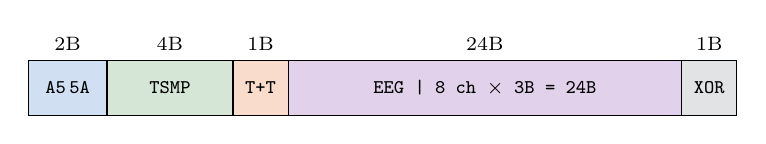
\begin{tikzpicture}[
    field/.style={draw, minimum height=0.7cm, font=\scriptsize\ttfamily, anchor=west},
    lbl/.style={font=\scriptsize, anchor=south}
]
    % --- EEG-only (32B) ---
    \def\x{0}
    \node[field, fill=hwcolor!20, minimum width=1.0cm] (h) at (\x,0) {A5\,5A};
    \node[lbl] at (h.north) {2B};
    \pgfmathsetmacro{\x}{\x+1.0}
    \node[field, fill=fwcolor!20, minimum width=1.6cm] (ts) at (\x,0) {TSMP};
    \node[lbl] at (ts.north) {4B};
    \pgfmathsetmacro{\x}{\x+1.6}
    \node[field, fill=conncolor!20, minimum width=0.7cm] (ty) at (\x,0) {T+T};
    \node[lbl] at (ty.north) {1B};
    \pgfmathsetmacro{\x}{\x+0.7}
    \node[field, fill=plugincolor!20, minimum width=5.0cm] (eeg) at (\x,0) {EEG — 8 ch $\times$ 3B = 24B};
    \node[lbl] at (eeg.north) {24B};
    \pgfmathsetmacro{\x}{\x+5.0}
    \node[field, fill=extcolor!15, minimum width=0.7cm] (chk) at (\x,0) {XOR};
    \node[lbl] at (chk.north) {1B};
\end{tikzpicture}
\caption{EEG-only packet (Type \hex{00}) — 32 bytes, $\sim$80\% of traffic.}
\label{fig:eeg-only-packet}
\end{figure}

\begin{figure}[H]
\centering
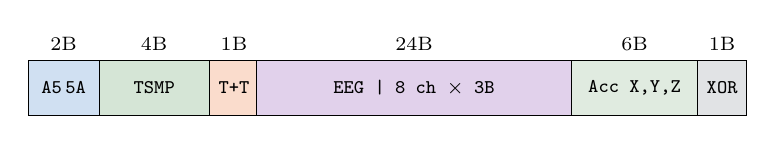
\begin{tikzpicture}[
    field/.style={draw, minimum height=0.7cm, font=\scriptsize\ttfamily, anchor=west},
    lbl/.style={font=\scriptsize, anchor=south}
]
    % --- EEG + Accel (38B) ---
    \def\x{0}
    \node[field, fill=hwcolor!20, minimum width=0.9cm] (h) at (\x,0) {A5\,5A};
    \node[lbl] at (h.north) {2B};
    \pgfmathsetmacro{\x}{\x+0.9}
    \node[field, fill=fwcolor!20, minimum width=1.4cm] (ts) at (\x,0) {TSMP};
    \node[lbl] at (ts.north) {4B};
    \pgfmathsetmacro{\x}{\x+1.4}
    \node[field, fill=conncolor!20, minimum width=0.6cm] (ty) at (\x,0) {T+T};
    \node[lbl] at (ty.north) {1B};
    \pgfmathsetmacro{\x}{\x+0.6}
    \node[field, fill=plugincolor!20, minimum width=4.0cm] (eeg) at (\x,0) {EEG — 8 ch $\times$ 3B};
    \node[lbl] at (eeg.north) {24B};
    \pgfmathsetmacro{\x}{\x+4.0}
    \node[field, fill=fwcolor!15, minimum width=1.6cm] (acc) at (\x,0) {Acc X,Y,Z};
    \node[lbl] at (acc.north) {6B};
    \pgfmathsetmacro{\x}{\x+1.6}
    \node[field, fill=extcolor!15, minimum width=0.6cm] (chk) at (\x,0) {XOR};
    \node[lbl] at (chk.north) {1B};
\end{tikzpicture}
\caption{EEG + Accelerometer packet (Type \hex{01}) — 38 bytes, largest packet.}
\label{fig:eeg-accel-packet}
\end{figure}

\subsection{TYPE+TTL Byte}
\label{sec:type-ttl}

Offset~6 packs TTL trigger lines and packet type into 8~bits:

\begin{figure}[H]
\centering
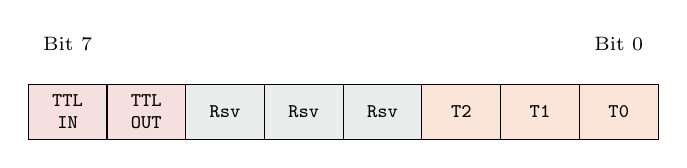
\begin{tikzpicture}[
    bit/.style={draw, minimum width=1.0cm, minimum height=0.7cm,
                font=\scriptsize\ttfamily, align=center}
]
    \node[bit, fill=oecolor!15] (b7) at (0,0) {TTL\\IN};
    \node[bit, fill=oecolor!15] (b6) at (1,0) {TTL\\OUT};
    \node[bit, fill=extcolor!10] (b5) at (2,0) {Rsv};
    \node[bit, fill=extcolor!10] (b4) at (3,0) {Rsv};
    \node[bit, fill=extcolor!10] (b3) at (4,0) {Rsv};
    \node[bit, fill=conncolor!15] (b2) at (5,0) {T2};
    \node[bit, fill=conncolor!15] (b1) at (6,0) {T1};
    \node[bit, fill=conncolor!15] (b0) at (7,0) {T0};

    \node[above=0.3cm, font=\scriptsize] at (b7.north) {Bit 7};
    \node[above=0.3cm, font=\scriptsize] at (b0.north) {Bit 0};
\end{tikzpicture}
\caption{TYPE+TTL byte bit-field layout.  Bit~7 = MSB, Bit~0 = LSB.}
\label{fig:type-ttl-byte}
\end{figure}

\begin{table}[H]
\centering
\caption{TYPE+TTL bit assignments}
\label{tab:type-ttl-bits}
\begin{tabularx}{\textwidth}{c l X}
\toprule
\textbf{Bit(s)} & \textbf{Name} & \textbf{Description} \\
\midrule
7   & TTL\_IN   & External trigger input (1 = active) \\
6   & TTL\_OUT  & External trigger output (1 = active) \\
5--3 & Reserved & Must be \texttt{000} for normal packets; \texttt{111} = error signal \\
2--0 & TYPE     & Packet type selector (0--7, see \cref{tab:aux-blocks}) \\
\bottomrule
\end{tabularx}
\end{table}

\begin{table}[H]
\centering
\caption{Type codes (bits 2--0 of TYPE+TTL byte)}
\label{tab:type-codes}
\begin{tabularx}{\textwidth}{c c l X c}
\toprule
\textbf{Binary} & \textbf{Hex} & \textbf{Name} & \textbf{Auxiliary Data} & \textbf{Size} \\
\midrule
\texttt{000} & \hex{00} & \texttt{EEG}       & None               & 32\,B \\
\texttt{001} & \hex{01} & \texttt{EEG\_ACCEL} & Accelerometer (6\,B) & 38\,B \\
\texttt{010} & \hex{02} & \texttt{EEG\_PPG}   & PPG + SpO$_2$ (4\,B) & 36\,B \\
\texttt{011} & \hex{03} & \texttt{EEG\_TEMP}  & Temperature (2\,B)   & 34\,B \\
\texttt{100} & \hex{04} & \texttt{EEG\_BAT}   & Battery level (1\,B) & 33\,B \\
\texttt{101} & \hex{05} & \texttt{RESERVED\_1} & Future use          & --- \\
\texttt{110} & \hex{06} & \texttt{RESERVED\_2} & Future use          & --- \\
\texttt{111} & \hex{07} & \texttt{RESERVED\_3} & Future use          & --- \\
\bottomrule
\end{tabularx}
\end{table}

\subsubsection{TTL Examples}

\begin{table}[H]
\centering
\caption{Example TYPE+TTL byte values}
\label{tab:ttl-examples}
\begin{tabular}{l l l l l}
\toprule
\textbf{Hex} & \textbf{Binary} & \textbf{TTL} & \textbf{Type} & \textbf{Meaning} \\
\midrule
\hex{00} & \texttt{00|000|000} & ---     & EEG   & EEG only, no trigger \\
\hex{80} & \texttt{10|000|000} & IN      & EEG   & EEG only, TTL input active \\
\hex{C1} & \texttt{11|000|001} & IN+OUT  & ACCEL & EEG + Accel, both triggers \\
\hex{02} & \texttt{00|000|010} & ---     & PPG   & EEG + PPG + SpO$_2$, no trigger \\
\hex{43} & \texttt{01|000|011} & OUT     & TEMP  & EEG + Temp, TTL output active \\
\hex{84} & \texttt{10|000|100} & IN      & BAT   & EEG + Battery, TTL input active \\
\bottomrule
\end{tabular}
\end{table}

\subsubsection{Error Signalling}

When bits~5--3 are all set (\texttt{111}), the packet signals an
\textbf{error condition}: header with error flag + zeroed EEG data.

\begin{lstlisting}
A55A + TIMESTAMP(4B) + Error-flagged TYPE+TTL + 24x0x00 + CHECKSUM
\end{lstlisting}

\noindent Upon receiving an error packet, the host must:
\begin{enumerate}
    \item Stop acquisition.
    \item Return to handshake state.
    \item Report the error to the user.
\end{enumerate}

\subsection{Byte Offset Reference}

\begin{table}[H]
\centering
\caption{Absolute byte offsets for all active packet types (8-channel EEG)}
\label{tab:byte-offsets}
\begin{tabular}{l c c c c c}
\toprule
\textbf{Block} & \textbf{\hex{00} EEG} & \textbf{\hex{01} +Accel}
               & \textbf{\hex{02} +PPG} & \textbf{\hex{03} +Temp}
               & \textbf{\hex{04} +Bat} \\
\midrule
Sync (2\,B)       & 0--1  & 0--1  & 0--1  & 0--1  & 0--1  \\
Timestamp (4\,B)  & 2--5  & 2--5  & 2--5  & 2--5  & 2--5  \\
Type+TTL (1\,B)   & 6     & 6     & 6     & 6     & 6     \\
EEG (24\,B)       & 7--30 & 7--30 & 7--30 & 7--30 & 7--30 \\
Aux data          & ---   & 31--36 & 31--34 & 31--32 & 31   \\
Checksum (1\,B)   & 31    & 37    & 35    & 33    & 32    \\
\midrule
\textbf{Total}    & 32\,B & 38\,B & 36\,B & 34\,B & 33\,B \\
\bottomrule
\end{tabular}
\end{table}

\subsection{Multi-Rate Sensor Scheduling}

Every packet contains fresh 1000\,Hz EEG data.  Auxiliary sensors run at
sub-rates; collisions are resolved by \textbf{deferring lower-priority
sensors by 1\,ms} (the deferred packet still carries a fresh EEG sample).

\begin{table}[H]
\centering
\caption{Sensor scheduling rates}
\label{tab:sensor-schedule}
\begin{tabular}{l c c l}
\toprule
\textbf{Sensor} & \textbf{Rate (Hz)} & \textbf{Every $N$th pkt} & \textbf{Priority} \\
\midrule
EEG (+ TTL)        & 1000 & Every packet   & (always present) \\
Accelerometer      & 200  & Every 5th      & Highest \\
PPG + SpO$_2$      & 100  & Every 10th     & 2nd \\
Temperature        & 1    & Every 1000th   & 3rd \\
Battery            & 1    & Every 1000th   & Lowest \\
\bottomrule
\end{tabular}
\end{table}

\subsubsection{Collision Resolution}

Priority order (highest first):

\begin{center}
\texttt{ACCEL > PPG > TEMP > BAT}
\end{center}

\noindent Temperature and Battery (both 1\,Hz) are staggered so only one
is due at any given second boundary.

\subsubsection{Example: 21 Consecutive Packets}

\begin{lstlisting}[caption={Scheduling over 21 samples (Accel every 5th, PPG every 10th)}]
Pkt:  1    2    3    4    5     6    7    8    9    10
EEG: [EEG] [EEG] [EEG] [EEG] [EEG] [EEG] [EEG] [EEG] [EEG] [EEG]
Aux:  ---   ---   ---   ---  ACCEL  ---   ---   ---   ---  ACCEL
Size: 32B   32B   32B   32B   38B   32B   32B   32B   32B   38B

Pkt:  11   12   13   14    15   16   17   18   19    20    21
EEG: [EEG] [EEG] [EEG] [EEG] [EEG] [EEG] [EEG] [EEG] [EEG] [EEG] [EEG]
Aux:  PPG   ---   ---   ---  ACCEL  ---   ---   ---   ---  ACCEL  PPG
Size: 36B   32B   32B   32B   38B   32B   32B   32B   32B   38B   36B
\end{lstlisting}

\noindent PPG at pkt~10 defers to pkt~11 (Accel has priority); PPG at
pkt~20 defers to pkt~21.  Each deferred packet carries fresh EEG.
\fi
% END firmware comment-out

\subsection{LSL Stream Metadata Reference}

The Qt Connector Application publishes two LSL streams per device:

\begin{table}[H]
\centering
\caption{LSL StreamInfo constructor parameters}
\label{tab:lsl-streaminfo}
\begin{tabularx}{\textwidth}{l l l X}
\toprule
\textbf{Property} & \textbf{EEG Stream} & \textbf{Marker Stream} & \textbf{Notes} \\
\midrule
name            & \texttt{"InEarEEG"}           & \texttt{"InEarEEG\_Markers"} & Unique per device on network \\
type            & \texttt{"EEG"}                & \texttt{"Markers"}           & Enables LabRecorder / BIDS auto-detect \\
channel\_count  & 8                             & 1                            & 8 EEG channels; 1 event channel \\
nominal\_srate  & 1000.0                        & 0                            & 0 = \texttt{IRREGULAR\_RATE} \\
channel\_format & \texttt{cf\_float32}          & \texttt{cf\_string}          & $\mu$V for EEG; labels for markers \\
source\_id      & \texttt{"inear\_001"}         & \texttt{"inear\_001\_markers"} & Stable across sessions \\
\bottomrule
\end{tabularx}
\end{table}

% =============================================================================
\section{Layer 3 — Connector Applications}
\label{sec:connector}
% =============================================================================

The \component{LSL Connector Application} is the \textbf{primary production
connector} — a standalone Qt desktop app that bridges Teensy hardware to
LSL, completely independent of Open Ephys or any other recording software.

\begin{figure}[H]
\centering
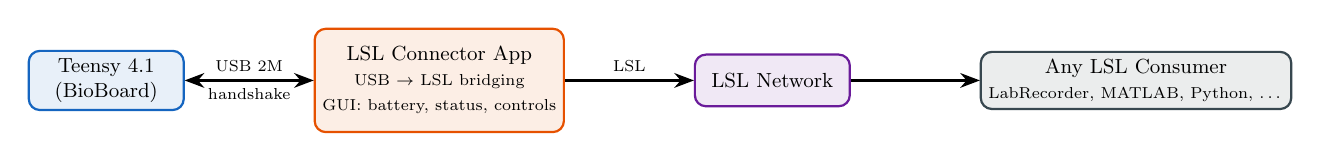
\begin{tikzpicture}[scale=0.82, every node/.style={transform shape},
    node distance=0.8cm and 1.6cm,
    box/.style={draw, rounded corners, thick, minimum width=2.4cm,
                minimum height=0.8cm, align=center, font=\small},
    arr/.style={-{Stealth[length=2.5mm]}, thick},
    darr/.style={{Stealth[length=2.5mm]}-{Stealth[length=2.5mm]}, thick}
]
    \node[box, fill=hwcolor!10, draw=hwcolor]  (teensy) {Teensy 4.1\\(BioBoard)};
    \node[box, fill=conncolor!10, draw=conncolor, right=2cm of teensy,
          minimum width=3.4cm, minimum height=1.6cm]
          (app) {LSL Connector App\\{\scriptsize USB $\to$ LSL bridging}\\{\scriptsize GUI: battery, status, controls}};
    \node[box, fill=plugincolor!10, draw=plugincolor, right=2cm of app]
          (lsl) {LSL Network};
    \node[box, fill=extcolor!10, draw=extcolor, right=2cm of lsl]
          (any) {Any LSL Consumer\\{\scriptsize LabRecorder, MATLAB, Python, \ldots}};

    \draw[darr] (teensy) -- node[above, font=\scriptsize] {USB 2M}
                            node[below, font=\scriptsize] {handshake} (app);
    \draw[arr]  (app)    -- node[above, font=\scriptsize] {LSL} (lsl);
    \draw[arr]  (lsl)    -- (any);
\end{tikzpicture}
\caption{LSL Connector Application data flow with two-way USB handshake.}
\label{fig:lsl-connector-app}
\end{figure}

\subsection{Minimum Viable Product (MVP)}

\paragraph{User Interface}

\begin{enumerate}
    \item \textbf{Scan Button} — Searches for connected Teensy devices
          (vendor/product ID filtering).
    \item \textbf{Stream Controls} — ``Open LSL'' / ``Close LSL'' toggle.
    \item \textbf{Status Display} — Battery level, connection state,
          stream health.
\end{enumerate}

\paragraph{Core Connectivity \& Data Flow}

\begin{enumerate}
    \item \textbf{USB Scanning} — Enumerates ports, filters by Teensy IDs.
    \item \textbf{Protocol Parsing} — Demultiplexes incoming serial stream
          per the Compact Protocol.
    \item \textbf{LSL Bridging} — Pushes parsed samples into an LSL outlet
          with correct metadata.
\end{enumerate}

\paragraph{Two-Way Communication \& Handshake Protocol}

A structured 4-step handshake precedes data streaming:

\begin{table}[H]
\centering
\caption{Handshake protocol steps}
\label{tab:handshake-steps}
\begin{tabularx}{\textwidth}{c l X}
\toprule
\textbf{Step} & \textbf{Phase} & \textbf{Description} \\
\midrule
1 & Device Recognition
  & Ping/response to confirm Teensy hardware identity. \\
2 & Firmware Recognition
  & Version query; mismatched versions trigger a warning. \\
3 & Pairing Handshake
  & Establishes exclusive session with the specific Teensy. \\
4 & Information Exchange
  & Dynamic retrieval of device configuration:
    \begin{itemize}[nosep, leftmargin=1em]
        \item Required number of LSL channels
        \item Battery status and charge level
        \item Sensor metadata (which sensors are present)
        \item Current sample rate and gain settings
    \end{itemize} \\
\bottomrule
\end{tabularx}
\end{table}

\paragraph{Error \& Special Situation Handling}

\begin{table}[H]
\centering
\caption{Error handling requirements}
\label{tab:error-handling}
\begin{tabularx}{\textwidth}{l X}
\toprule
\textbf{Condition} & \textbf{Required Behaviour} \\
\midrule
USB disconnect / timeout
    & Detect within 500\,ms; auto-pause LSL; attempt reconnect
      with exponential back-off. \\
Malformed packets
    & Discard (checksum failure); increment error counter; continue
      streaming valid data. \\
Buffer overruns
    & Drop oldest samples when ring buffer exceeds capacity; log
      warning with drop count. \\
Hardware failure flags
    & Parse Teensy error codes; display with severity colour coding;
      optionally pause on critical errors. \\
\bottomrule
\end{tabularx}
\end{table}

\subsection{Future Roadmap}

\paragraph{Expanded Hardware Support}

\begin{itemize}
    \item \textbf{SD Card Access} — Read/manage SD card files via Teensy USB.
    \item \textbf{Bluetooth} — Wireless streaming via RFCOMM/SPP transport.
\end{itemize}

\paragraph{UI Enhancements}

\begin{itemize}
    \item \textbf{Connection Toggle} — Seamless USB/Bluetooth switching.
    \item \textbf{Multi-device support} — Simultaneous connections, each
          with its own LSL outlet.
    \item \textbf{Config persistence} — Save/load device profiles.
\end{itemize}



% =============================================================================
\section{Layer 4 — Consumer Software \& Open Ephys Plugins}
\label{sec:plugins}
% =============================================================================

The LSL streams from the Qt Connector App can be consumed by any
LSL-compatible software (OpenBCI GUI, MATLAB, LabRecorder, Python scripts,
or any \texttt{liblsl} binding).  For \textbf{Open Ephys} users, in-house
C++ plugins provide enhanced integration on top of the LSL-first workflow.

\subsection{Open Ephys Plugin Inventory (Optional Integrations)}

For users who prefer extended Open Ephys workflows, the following plugins are
available. The primary production path remains
Qt~Connector~App~$\to$~LSL~$\to$~Open~Ephys~(LSL inlet).

\begin{table}[H]
\centering
\caption{Complete plugin inventory (optional Open Ephys integrations)}
\label{tab:plugin-inventory}
\begin{tabularx}{\textwidth}{l l X}
\toprule
\textbf{Plugin} & \textbf{Type} & \textbf{Function} \\
\midrule
\multicolumn{3}{l}{\textbf{In-house plugins (written by us)}} \\
\addlinespace
InEar Teensy Source         & DataThread & Direct USB; Compact Protocol v1.0 (8-ch, 32--38\,B) \\
InEar Teensy Optimised      & DataThread & Direct USB; legacy variable 26--55\,B protocol \\
Custom IC Source            & DataThread & Generic serial IC reader (any protocol) \\
OpenBCI Cyton               & DataThread & Cyton/Daisy 8/16-ch wireless EEG \\
EDF File Source             & FileSource & EDF/BDF/EDF+/CSV file playback \\
LSL Outlet                  & Processor  & Standalone LSL streaming output \\
Paradigm Bridge             & Processor  & TCP experiment control + TTL injection \\
\addlinespace
\multicolumn{3}{l}{\textbf{Open Ephys community plugins (used as dependencies)}} \\
\addlinespace
Lab Streaming Layer I/O     & Mixed      & LSL inlet (source) + outlet (sink) \\
Record Node                 & Sink       & Binary / NWB / Open Ephys format recording \\
LFP Viewer                  & Visualiser & Real-time waveform display \\
File Reader                 & Source     & Built-in file playback (extended by EDF plugin) \\
\bottomrule
\end{tabularx}
\end{table}

\subsection{Source Plugins — Serial Data Reader (Legacy / Development)}

The InEar Teensy Source plugin is a \textbf{custom in-house plugin}
that reads serial data directly from the BioBoard over USB. It is kept for
legacy compatibility and low-level debugging, but is not part of the primary
production architecture (which uses the Qt Connector as the single parser).

\begin{figure}[H]
\centering
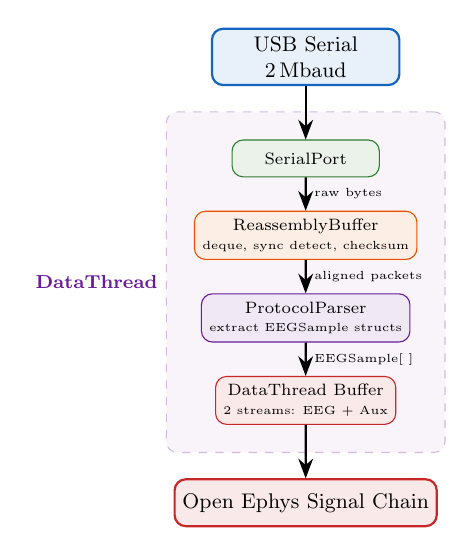
\begin{tikzpicture}[scale=0.85, every node/.style={transform shape},
    node distance=0.5cm and 0.3cm,
    box/.style={draw, rounded corners, thick, minimum width=2.8cm,
                minimum height=0.7cm, align=center, font=\small},
    comp/.style={draw, rounded corners, minimum width=2.2cm,
                 minimum height=0.55cm, align=center, font=\scriptsize},
    arr/.style={-{Stealth[length=2.5mm]}, thick}
]
    % USB input
    \node[box, fill=hwcolor!10, draw=hwcolor] (usb) {USB Serial\\2\,Mbaud};

    % SerialPort
    \node[comp, fill=fwcolor!10, draw=fwcolor, below=0.8cm of usb]
         (sp) {SerialPort};

    % ReassemblyBuffer
    \node[comp, fill=conncolor!10, draw=conncolor, below=0.5cm of sp]
         (rb) {ReassemblyBuffer\\{\tiny deque, sync detect, checksum}};

    % ProtocolParser
    \node[comp, fill=plugincolor!10, draw=plugincolor, below=0.5cm of rb]
         (pp) {ProtocolParser\\{\tiny extract EEGSample structs}};

    % DataThread buffer
    \node[comp, fill=oecolor!10, draw=oecolor, below=0.5cm of pp]
         (dt) {DataThread Buffer\\{\tiny 2 streams: EEG + Aux}};

    % Open Ephys
    \node[box, fill=oecolor!10, draw=oecolor, below=0.8cm of dt]
         (oe) {Open Ephys Signal Chain};

    % Arrows
    \draw[arr] (usb) -- (sp);
    \draw[arr] (sp)  -- node[right, font=\tiny] {raw bytes} (rb);
    \draw[arr] (rb)  -- node[right, font=\tiny] {aligned packets} (pp);
    \draw[arr] (pp)  -- node[right, font=\tiny] {EEGSample[ ]} (dt);
    \draw[arr] (dt)  -- (oe);

    % Surrounding box
    \begin{scope}[on background layer]
        \node[fit=(sp)(rb)(pp)(dt), inner sep=10pt, fill=plugincolor!5,
              draw=plugincolor!30, dashed, rounded corners,
              label={[plugincolor, font=\footnotesize\bfseries]left:DataThread}] {};
    \end{scope}
\end{tikzpicture}
\caption{Internal architecture of the InEar Teensy source plugin.}
\label{fig:datathread-arch}
\end{figure}

\subsubsection{Packet Reassembly}

USB transfers arrive in arbitrary-sized chunks.  The \component{Reassembly\-Buffer}
uses a \texttt{std::deque\allowbreak<uint8\_t>} to:

\begin{enumerate}
    \item Scan for sync word~\hex{A5\,5A}.
    \item Read expected length from TYPE+TTL byte.
    \item Validate XOR checksum.
    \item Extract validated packet; discard pre-sync bytes.
    \item Detect lost packets via timestamp gaps.
\end{enumerate}

\subsubsection{Output Data Streams}

Each source plugin registers \textbf{two data streams} with Open Ephys:

\begin{table}[H]
\centering
\begin{tabular}{l c c l}
\toprule
\textbf{Stream} & \textbf{Channels} & \textbf{Rate} & \textbf{Contents} \\
\midrule
EEG  & 8  & 1000\,Hz & Channels 1--8, scaled to $\mu$V \\
Aux  & varies & 1000\,Hz & Accel, PPG+SpO$_2$, Temp, Battery (sample-and-hold) \\
\bottomrule
\end{tabular}
\end{table}

\subsubsection{Simulation Mode}

Both source plugins include simulation mode (toggled in editor UI):

\begin{itemize}
    \item \textbf{EEG:} Sine waves at 3, 7, 11, 15, 19\,Hz (one per channel)
    \item \textbf{PPG:} 72\,BPM synthetic waveform with Red/IR/Green variations
    \item \textbf{Accel:} Slow sinusoidal motion
    \item \textbf{Sync:} Xorshift32 PRNG-driven digital pulse
\end{itemize}


\subsection{OpenBCI Cyton Plugin}

The system also supports the \textbf{OpenBCI Cyton} board (8-channel
wireless EEG):

\begin{table}[H]
\centering
\caption{OpenBCI Cyton vs.\ BioBoard comparison}
\label{tab:cyton-vs-bioboard}
\begin{tabularx}{\textwidth}{l X X}
\toprule
\textbf{Feature} & \textbf{BioBoard (InEar)} & \textbf{OpenBCI Cyton} \\
\midrule
ADC            & ADS1299 (same chip)         & ADS1299 (same chip) \\
Channels       & 8 EEG + aux (Accel, PPG, Temp, Bat) & 8 EEG (+8 Daisy) + 3 accel \\
Sample rate    & 1000\,Hz                     & 250\,Hz \\
Connection     & USB wired, 2\,Mbaud          & 2.4\,GHz radio, 115\,200\,baud \\
Packet size    & 32--38\,B (Compact Protocol)  & 33\,B \\
Extra sensors  & PPG+SpO$_2$, Temp, Battery   & Accelerometer only \\
\bottomrule
\end{tabularx}
\end{table}


\subsection{Paradigm Bridge — Experiment Control}
\label{sec:paradigm-bridge}

The \component{Paradigm Bridge} is a \textbf{filter processor} providing
bidirectional TCP control between experiment software (PsychoPy, MATLAB)
and Open Ephys.

\begin{figure}[H]
\centering
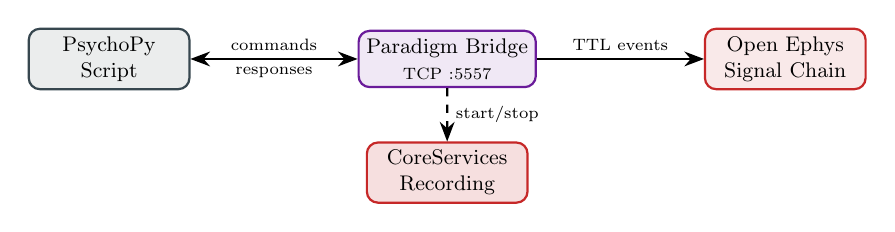
\begin{tikzpicture}[scale=0.85, every node/.style={transform shape},
    node distance=0.8cm and 2cm,
    box/.style={draw, rounded corners, thick, minimum width=2.4cm,
                minimum height=0.8cm, align=center, font=\small},
    arr/.style={-{Stealth[length=2.5mm]}, thick},
    darr/.style={{Stealth[length=2.5mm]}-{Stealth[length=2.5mm]}, thick}
]
    \node[box, fill=extcolor!10, draw=extcolor] (ps) {PsychoPy\\Script};
    \node[box, fill=plugincolor!10, draw=plugincolor, right=2.5cm of ps]
          (pb) {Paradigm Bridge\\{\scriptsize TCP :5557}};

    \node[box, fill=oecolor!10, draw=oecolor, right=2.5cm of pb]
          (oe) {Open Ephys\\Signal Chain};

    \draw[darr] (ps) -- node[above, font=\scriptsize] {commands}
                        node[below, font=\scriptsize] {responses} (pb);
    \draw[arr]  (pb) -- node[above, font=\scriptsize] {TTL events} (oe);

    % Downward: recording control
    \node[box, fill=oecolor!15, draw=oecolor, below=0.8cm of pb]
          (rec) {CoreServices\\Recording};
    \draw[arr, dashed] (pb) -- node[right, font=\scriptsize] {start/stop} (rec);
\end{tikzpicture}
\caption{Paradigm Bridge bidirectional control flow.}
\label{fig:paradigm-bridge}
\end{figure}

\subsection{LSL Integration}

\begin{itemize}
    \item \textbf{LSL Inlet} (DataThread) — Receives any LSL stream as an
          Open Ephys source.
    \item \textbf{LSL Outlet} (Processor) — Streams data and markers from
          Open Ephys to external consumers.
\end{itemize}

\subsection{EDF File Source}

The \component{EDF File Source} extends the built-in File Reader to support
EDF, BDF, EDF+, CSV, and XZ-compressed CSV files for offline replay.


% =============================================================================
\section{Signal Chain Configurations}
\label{sec:signal-chains}
% =============================================================================

\subsection{Primary Path — Qt Connector App (Standalone)}

For users with or without Open Ephys:

\begin{lstlisting}
[BioBoard] -> USB -> [Qt Connector App] -> LSL network
                                             |
              +-------------+----------------+---------------------+
              |             |                |                     |
      [Open Ephys Inlet] [OpenBCI GUI] [LabRecorder]        [MATLAB/Python]
      (visualize/record)               (XDF file)

[PsychoPy / behavior scripts] -> LSL network (markers/events)
\end{lstlisting}

\subsection{Open Ephys Path — LSL Inlet + Optional LSL Outlet}

Open Ephys subscribes to the Connector App stream via LSL (no direct serial
parser in Open Ephys on the primary architecture), visualises/records
internally, and can optionally publish events/markers back to LSL:

\begin{lstlisting}
[BioBoard] -> USB -> [Qt Connector App] -> LSL network
                                             |
                                      [Open Ephys Inlet]
                                             |
              +------------------------+------------------------+
              |                        |                        |
        [LFP Viewer]   [Paradigm Bridge] -> [Record Node]   [LSL Outlet]
                                                                |
                                                            LSL network
                                                                |
                                            [LabRecorder] [MATLAB] [Python]
\end{lstlisting}

\subsection{Offline Replay with Annotations}

Replay a previously recorded EDF file with post-hoc annotation:

\begin{lstlisting}
[File Reader + EDF Source] -> [Paradigm Bridge] -> [LFP Viewer]
\end{lstlisting}

\subsection{Multi-Device with LSL}

Multiple BioBoards and/or third-party devices, each with their own
Qt Connector App instance:

\begin{lstlisting}
[BioBoard A] -> [Qt Connector App 1] -> LSL "InEarEEG_A"
[BioBoard B] -> [Qt Connector App 2] -> LSL "InEarEEG_B"   -> [LabRecorder]
[OpenBCI Cyton] -> [OpenBCI GUI] -----> LSL "OpenBCI"      -> [LabRecorder]
\end{lstlisting}


% =============================================================================
\section{Build System}
\label{sec:build}
% =============================================================================

All C++ plugins use the standard Open Ephys CMake template:

\begin{lstlisting}[language=bash, caption={Building a plugin}]
cd OEPlugins/<plugin-name>/Build
cmake -G "Visual Studio 17 2022" -A x64 ..
cmake --build . --config Release
cmake --install . --config Release
# DLL installed to: plugin-GUI/Build/Release/plugins/
\end{lstlisting}

\begin{table}[H]
\centering
\caption{Build requirements}
\begin{tabular}{l l}
\toprule
\textbf{Tool} & \textbf{Version} \\
\midrule
CMake                & $\geq$ 3.15 \\
Visual Studio        & 2022 (MSVC 17) \\
Open Ephys Plugin API & v10 \\
Open Ephys GUI       & v1.0.1 (plugin-GUI submodule) \\
\bottomrule
\end{tabular}
\end{table}


\end{document}
